\section{Unconstrained continuous optimization}

In the following we treat only unconstrained continuous optimization problems. In these we are looking for the minimum of a function $f: R^n \Rightarrow R$ over \textbf{all} points $\overrightarrow{x} \in R^n$ for which $f(\overrightarrow{x})$ is defined.

\begin{figure}[H]
\centering
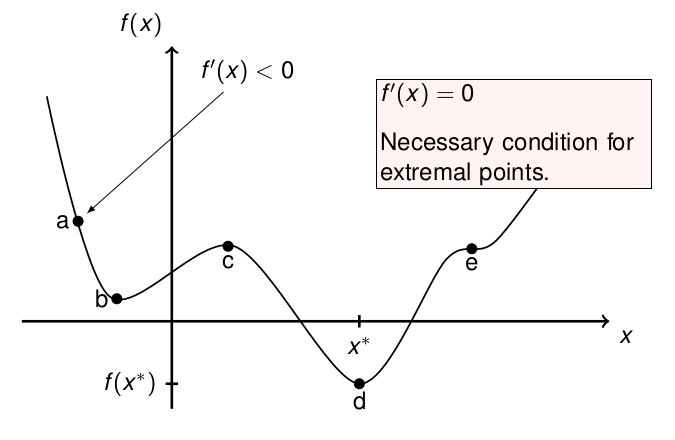
\includegraphics[width=0.6\textwidth]{figures/one-dimensional-optimization.png}
\caption{One dimensional optimization example}
\end{figure}

The gradient $ \bigtriangledown f$ of the function $f: R^n \Rightarrow R$ is the vector consisting of the $n$ partial derivatives of the vector.

$\bigtriangledown f(\overrightarrow{x}) = \begin{vmatrix}
f_{x1}(\overrightarrow{x}) \\
f_{x2}(\overrightarrow{x})  \\
\vdots \\
f_{x1}(\overrightarrow{x})  \\
\end{vmatrix}$
\\
\\
At each point $\overrightarrow{x}$ , the gradient $\bigtriangledown f(\overrightarrow{x})$ points in the direction of steepest ascent.
Its norm $||\bigtriangledown f(\overrightarrow{x})||$ gives the slope in that direction.

If all $x$ in $\bigtriangledown f(\overrightarrow{x}) = 0$, we have a stationary point in $f$. This doesn't mean that we have a extremal point, because there are also stationary points like e in the figure on top.

\clearpage
\subsection{Gradient Descent}
Gradient descent is an algorithm to find a local minimum of an (unconstrained multidimensional smooth) function f.
The function increases in direction of the gradient, so by going in the opposite direction we will get decreasing function values.

Algorithm:
\begin{itemize}
    \item Initialization: Choose starting point $x^0$
    \item Iteration step $x^i \Rightarrow x^{i+1}$: \\
    Determine local gradient $\bigtriangledown f(x^i)$ and move by some amount $\beta$ in opposite direction $\Rightarrow$ new point $x^{i+1}$. \\
    Repeat until gradient is (approximately) zero / no more (significant) decreases of the function values are observed.
\end{itemize}

\textbf{But} what is the optimal Step size $\beta$ in $x^{i+1} = x^i - \beta \bigtriangledown f(x^i)$?

\subsubsection{Successive halving of the step size}
The second step in the following notes is an extension of the successive halfening of the step size.

\begin{figure}[H]
\centering
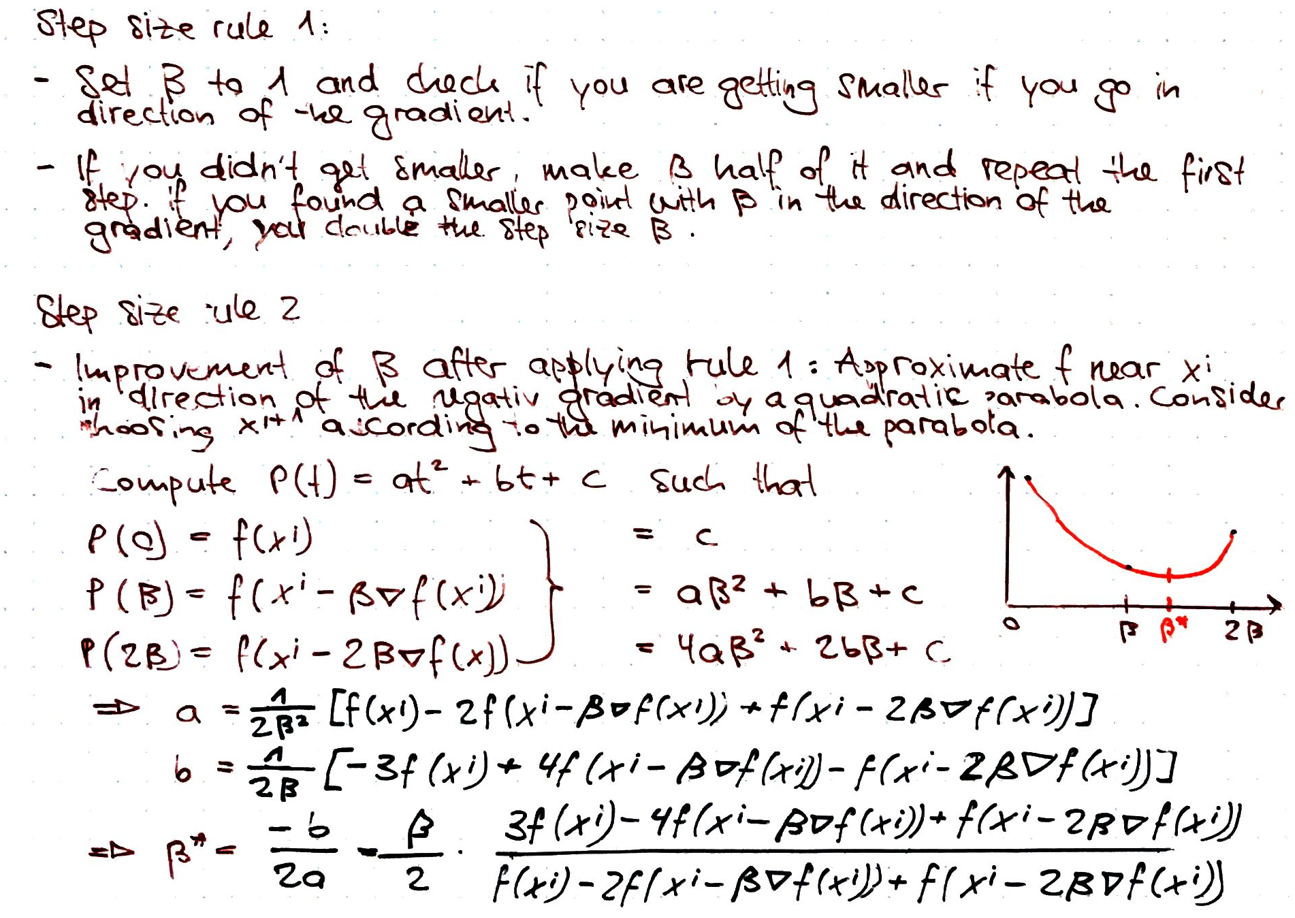
\includegraphics[width=1\textwidth]{figures/stepsizehalfening.png}
\caption{Successive halving of the step size}
\end{figure}

\subsection{Newton’s method}

\begin{figure}[H]
\centering
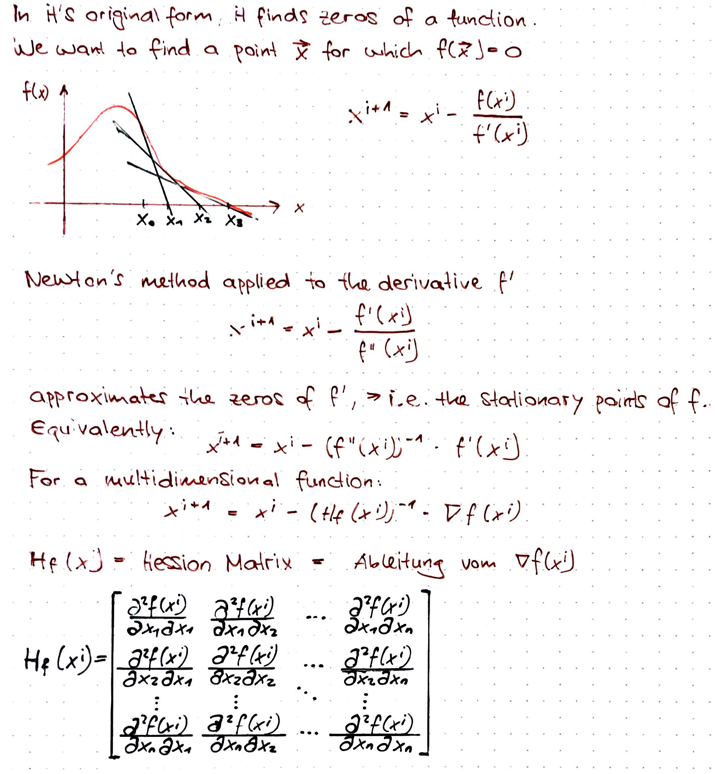
\includegraphics[width=1\textwidth]{figures/newtonMethod.png}
\caption{Newton’s method}
\end{figure}

\begin{enumerate}
    \item Initialization: \\
    Choose starting point $x^0$
    \item Iteration step $x^i \Rightarrow x^{i+1}$: \\
    $x^{i+1} = x^i - H_f(x^i)^{-1} \bigtriangledown f(x^i)$ 
    \item Repeat iteration step until break condition is met.
\end{enumerate}

\subsection{Speed of convergence}

\begin{figure}[H]
\centering
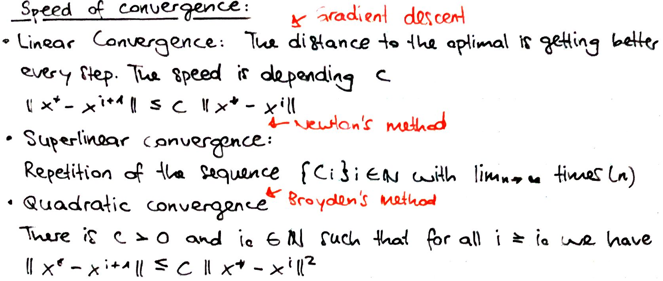
\includegraphics[width=0.9\textwidth]{figures/speedConvergence.png}
\caption{Continuous Optimization - Speed of convergence}
\end{figure}

\subsection{Approximating partial derivatives}

\begin{figure}[H]
\centering
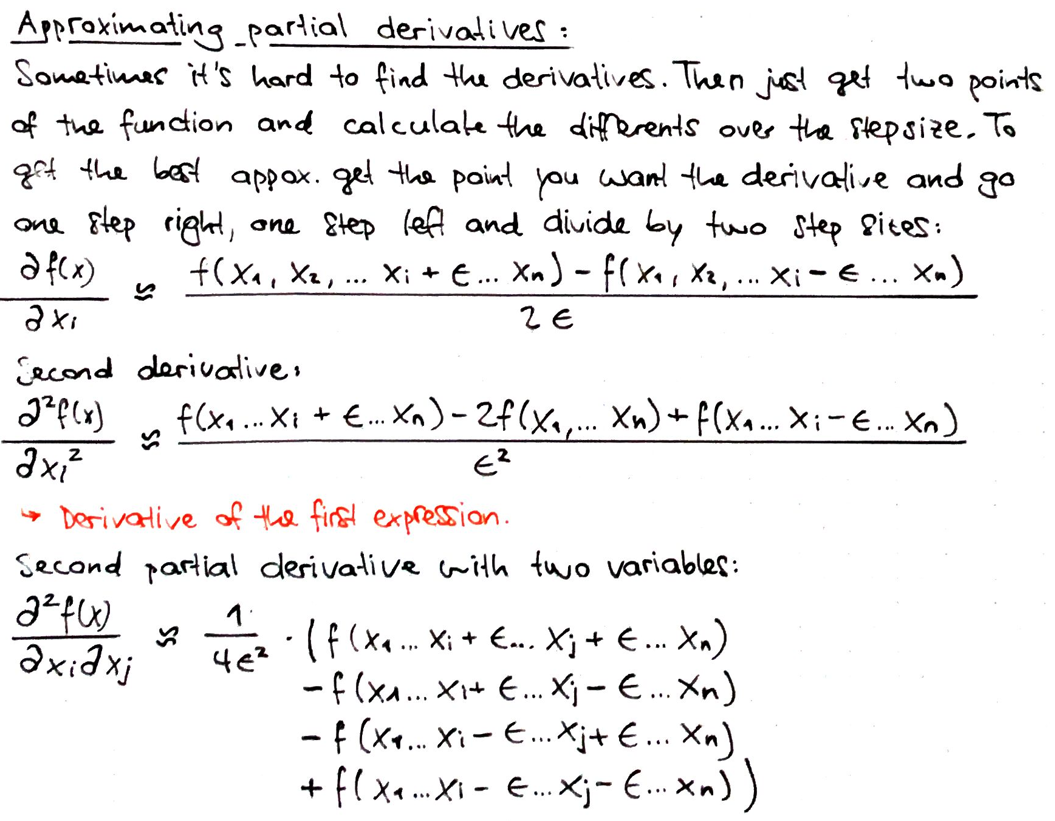
\includegraphics[width=0.9\textwidth]{figures/approxDerivatives.png}
\caption{Continuous Optimization - Approximating partial derivatives}
\end{figure}

\subsection{Broyden's method}
Computing and inverting the Hessian matrix $H_f (x^i)$ exactly in
the (approximate version of) Newton’s method is computationally expensive.
The idea in quasi-Newton methods is to approximate the inverse of the Hessian, $H_f (x^i)^-1$, by some matrix $(A_i)^{-1}$ that can be computed more efficiently.

Broyden’s method is a prominent example of a quasi-Newton
method, where you aproximate the ”derivative of the derivative”.

\begin{figure}[H]
\centering
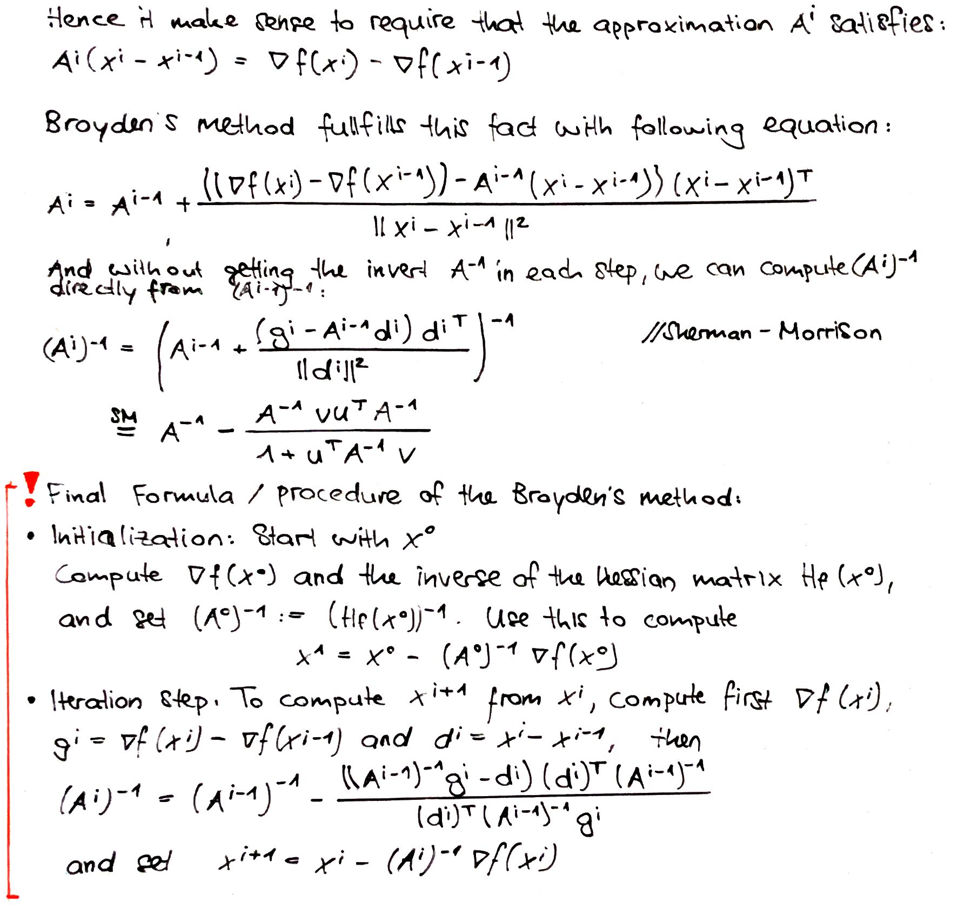
\includegraphics[width=1\textwidth]{figures/broyden.png}
\caption{Broyden's method}
\end{figure}

\clearpage
\subsection{Aitken's acceleration method}
To conclude, we present a general approach that can be used to improve the convergence speed of other methods (e.g. of the ones presented so far).
Aitken’s method is not a new method for finding local extrema, but can be used to improve the convergence speed of other existing methods that would converge slowly otherwise.

\begin{figure}[H]
\centering
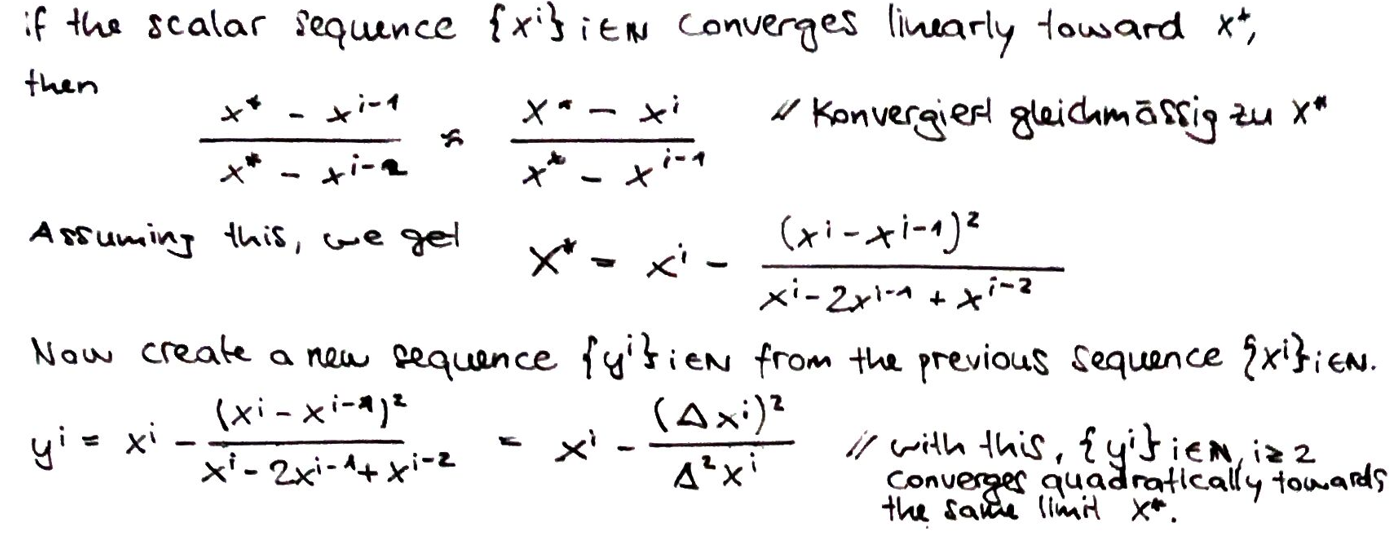
\includegraphics[width=1\textwidth]{figures/aitken.png}
\caption{Aitken's method}
\end{figure}

\clearpage